\documentclass[11pt,letterpaper]{article}

\usepackage[letterpaper,margin=0.90in,top=0.82in,bottom=0.82in,
            headheight=27pt,headsep=16pt,footskip=28pt]{geometry}
\usepackage[T1]{fontenc}
\usepackage[utf8]{inputenc}
\usepackage{mathpazo}
\usepackage[scaled=0.90]{helvet}
\usepackage{courier}
\usepackage{microtype}
\usepackage{amsmath,amssymb,mathtools,bm}
\usepackage{graphicx}
\usepackage{booktabs,tabularx,array}
\usepackage{caption}
\usepackage{float}
\usepackage{placeins}
\usepackage{enumitem}
\usepackage{listings}
\usepackage[most]{tcolorbox}
\usepackage{xcolor}
\usepackage{fancyhdr}
\usepackage{lastpage}
\usepackage{titlesec}
\usepackage[hidelinks]{hyperref}

\definecolor{nyupurple}{HTML}{57068C}
\definecolor{nyudark}{HTML}{2B1739}
\definecolor{nyulight}{HTML}{F4EFF8}
\definecolor{rulegray}{HTML}{C9C5CC}
\definecolor{textgray}{HTML}{5C5860}

\graphicspath{{../out/}}
\setlength{\parindent}{0pt}
\setlength{\parskip}{4.2pt plus 0.8pt minus 0.6pt}
\setlength{\emergencystretch}{2em}
\allowdisplaybreaks[2]

\titleformat{\section}
  {\Large\bfseries\color{nyupurple}}{}{0pt}{}
\titlespacing*{\section}{0pt}{16pt plus 3pt minus 2pt}{7pt}
\titleformat{\subsection}
  {\large\bfseries\color{nyudark}}{}{0pt}{}
\titlespacing*{\subsection}{0pt}{12pt plus 2pt minus 1pt}{4pt}
\titleformat{\subsubsection}
  {\normalsize\bfseries}{}{0pt}{}
\titlespacing*{\subsubsection}{0pt}{8pt plus 1pt}{2pt}

\captionsetup{
  font=small,
  labelfont={bf,color=nyupurple},
  textfont=it,
  justification=justified,
  singlelinecheck=false,
  skip=5pt
}

\newtcolorbox{resultbox}[1][]{
  enhanced,
  breakable,
  colback=nyulight,
  colframe=nyupurple!55,
  boxrule=0.6pt,
  arc=1.5pt,
  left=8pt,right=8pt,top=6pt,bottom=6pt,
  before skip=7pt,after skip=7pt,
  #1
}

\lstdefinestyle{output}{
  basicstyle=\ttfamily\small,
  backgroundcolor=\color{nyulight},
  frame=single,
  rulecolor=\color{nyupurple!45},
  framesep=7pt,
  xleftmargin=2pt,
  xrightmargin=2pt,
  columns=fullflexible,
  keepspaces=true,
  showstringspaces=false
}

\pagestyle{fancy}
\fancyhf{}
\fancyhead[L]{%
  \sffamily\fontsize{7.5}{9}\selectfont
  \textcolor{nyupurple}{\bfseries NEW YORK UNIVERSITY}\\[-1pt]
  \textcolor{textgray}{ELIGULI HAN}}
\fancyhead[R]{%
  \sffamily\fontsize{7.2}{9}\selectfont
  \textcolor{textgray}{COURANT INSTITUTE OF MATHEMATICAL SCIENCES}\\[-1pt]
  \textcolor{textgray}{HOMEWORK REPORT \;|\; PROBLEMS 1--4}}
\fancyfoot[L]{%
  \sffamily\fontsize{7}{8}\selectfont\textcolor{textgray}
  {PMF ESTIMATION \;|\; PARETO TAILS \;|\; KL DIVERGENCE}}
\fancyfoot[R]{%
  \sffamily\fontsize{7}{8}\selectfont\bfseries\textcolor{nyupurple}
  PAGE \thepage\ OF \pageref*{LastPage}}
\renewcommand{\headrulewidth}{0.8pt}
\renewcommand{\footrulewidth}{0.5pt}
\makeatletter
\renewcommand{\headrule}{%
  \hbox to\headwidth{\color{nyupurple}\leaders\hrule height \headrulewidth\hfill}}
\renewcommand{\footrule}{%
  \hbox to\headwidth{\color{rulegray}\leaders\hrule height \footrulewidth\hfill}}
\makeatother

\newcommand{\problem}[2]{\section*{#1. #2}}
\newcommand{\problemPart}[2]{\subsection*{#1\quad #2}}
\newcommand{\E}{\mathbb{E}}
\newcommand{\Var}{\operatorname{Var}}
\newcommand{\Prob}{\mathbb{P}}
\newcommand{\KL}{D_{\mathrm{KL}}}
\newcommand{\phat}{\widehat p}
\newcommand{\mhat}{\widehat m}
\newcommand{\alphahat}{\widehat\alpha}
\newcommand{\lambdahat}{\widehat\lambda}

\hypersetup{
  pdftitle={Tennis PMFs, Pareto Tails, Fires, and KL Divergence},
  pdfauthor={Eliguli Han},
  pdfsubject={NYU Mathematics Homework Report, Problems 1--4},
  pdfkeywords={probability mass function, Pareto distribution, maximum likelihood, KL divergence}
}

\begin{document}
\setcounter{figure}{-1}

\begin{center}
  {\sffamily\small\bfseries\color{nyupurple} MATHEMATICS HOMEWORK REPORT}\par
  \vspace{5pt}
  {\LARGE\bfseries Tennis PMFs, Pareto Tails, Fires,\\[2pt]
  and Kullback--Leibler Divergence}\par
  \vspace{5pt}
  {\large\color{textgray} Complete solutions, computational output, and visual verification}\par
\end{center}

\vspace{4pt}
\begin{tcolorbox}[
  colback=white,colframe=rulegray,boxrule=0.5pt,arc=0pt,
  left=8pt,right=8pt,top=5pt,bottom=5pt]
\begin{tabularx}{\linewidth}{@{}>{\sffamily\bfseries}l X >{\sffamily\bfseries}l X@{}}
Student: & Eliguli Han & Institution: & New York University \\
Document: & Problems 1--4 & Format: & Formal mathematical report
\end{tabularx}
\end{tcolorbox}

\section*{0. Reproducible computational output}

\begin{lstlisting}[style=output]
Total games in 6 matches: [39, 56, 45, 59, 40, 34]
Overall Alcaraz win prob on serve: 0.6251 (532/851)
Overall Sinner win prob on serve: 0.6191 (564/911)
Mean games: 41.72156
Min games: 21
Max games: 65
Alcaraz hold prob: 0.785655156946372
Sinner hold prob: 0.7741269513953015
Pooled: p_A = 0.6251, p_S = 0.6191
Mean of ratios: p_A = 0.6343, p_S = 0.6258
\end{lstlisting}

The simulation uses seed $42$ and $N=100{,}000$. The included regression checks reproduce the reference output exactly, while an independent dynamic-programming calculation validates the simulated pmf. The summary figure \texttt{tennis\_pmf\_comparison.png} is shown below.

\begin{figure}[H]
  \centering
  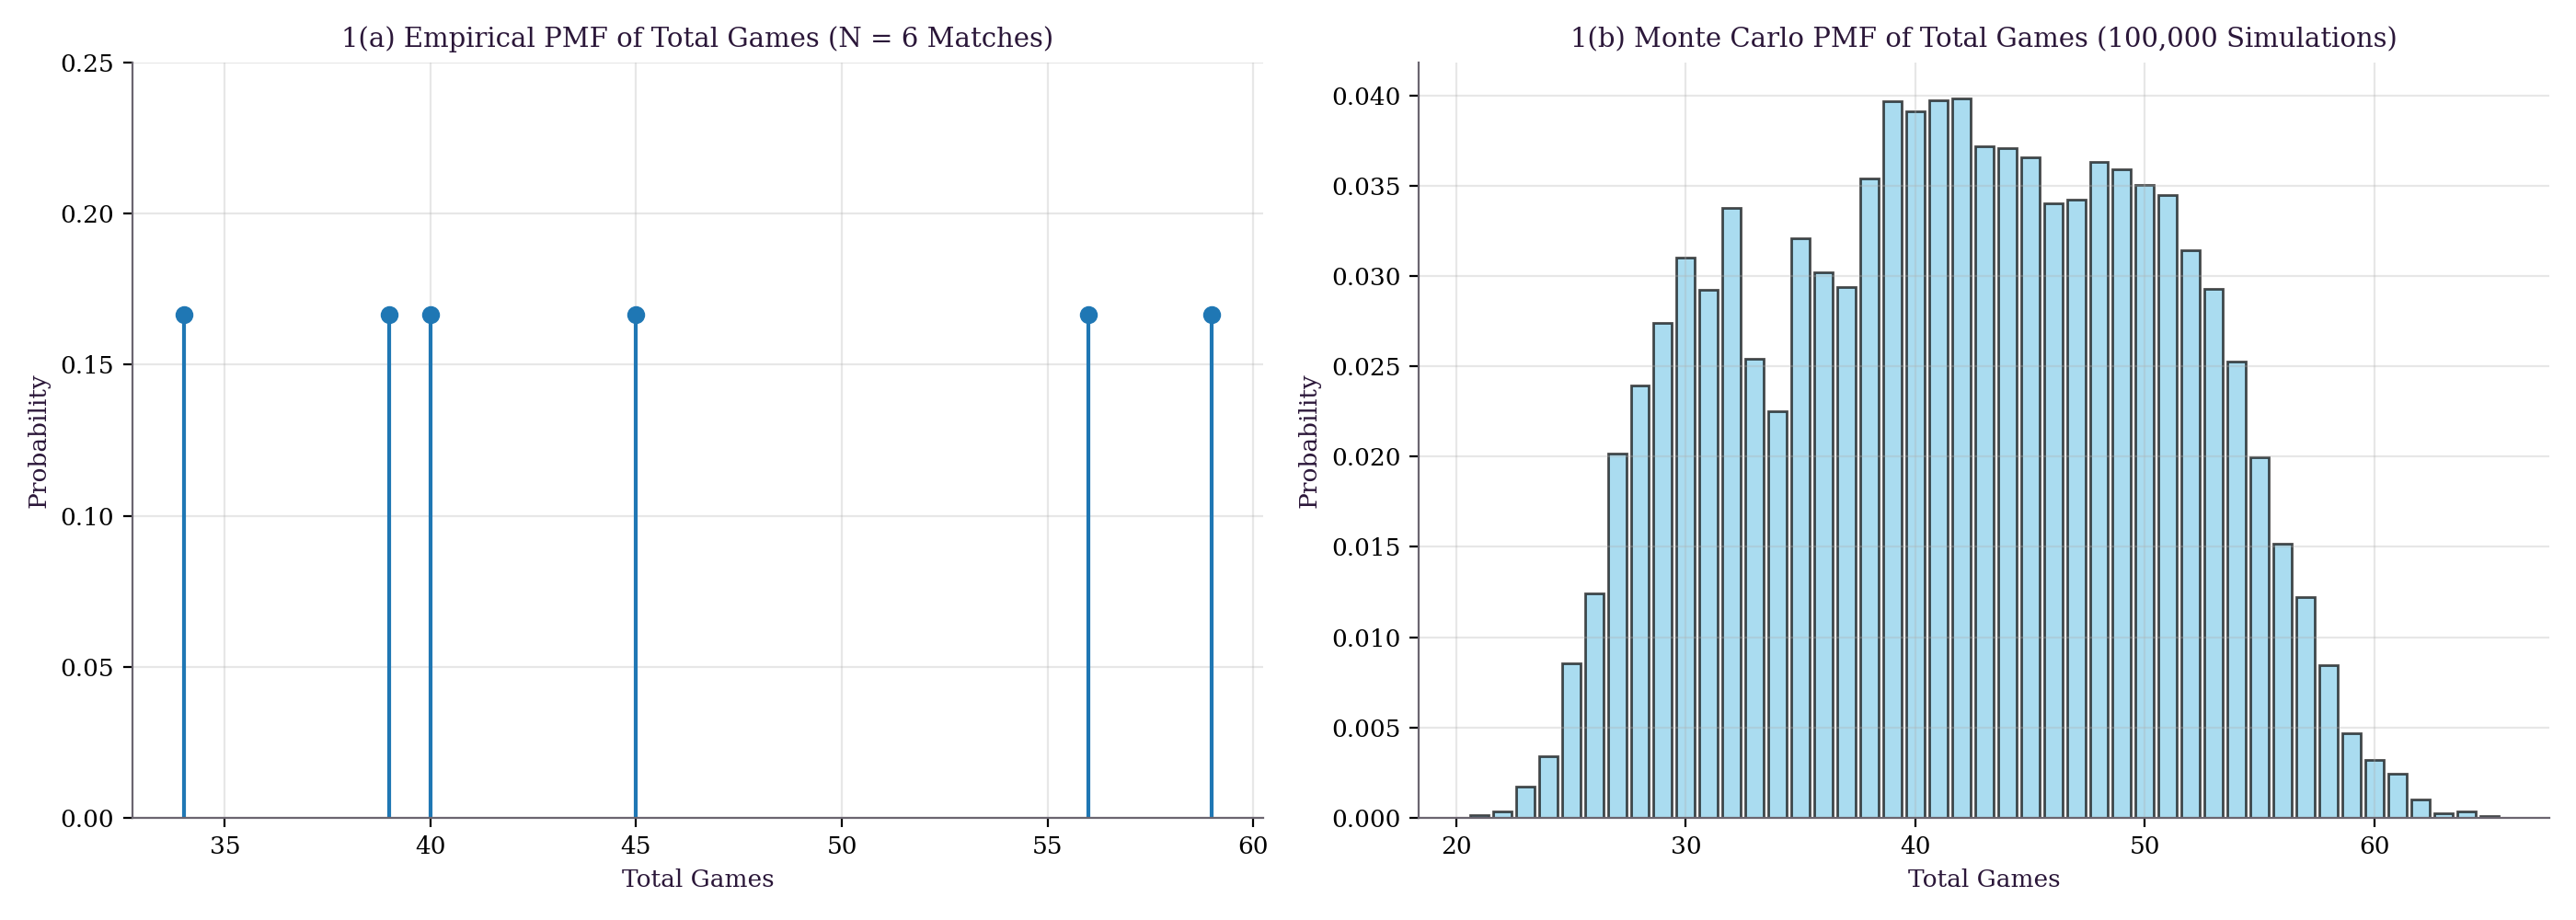
\includegraphics[width=\linewidth]{tennis_pmf_comparison.png}
  \caption{Empirical and Monte Carlo pmfs generated by the tennis simulation.}
  \label{fig:original-pmf}
\end{figure}

\begin{table}[H]
\centering
\caption{Match data. A tie-break set $(7\text{--}6)$ counts as 13 games.}
\label{tab:match-data}
\fontsize{8.6}{10.6}\selectfont
\begin{tabularx}{\linewidth}{@{}l >{\raggedright\arraybackslash}X c c r r@{}}
\toprule
Match & Set scores (Alcaraz--Sinner) & Sets & Games & Alcaraz serve & Sinner serve \\
\midrule
M1 & $1\text{--}6,\ 4\text{--}6,\ 7\text{--}6,\ 3\text{--}6$ & 4 & 39 & $76/121=0.628$ & $101/143=0.706$ \\
M2 & $6\text{--}3,\ 6\text{--}7,\ 6\text{--}7,\ 7\text{--}5,\ 6\text{--}3$ & 5 & 56 & $104/169=0.615$ & $118/213=0.554$ \\
M3 & $2\text{--}6,\ 6\text{--}3,\ 3\text{--}6,\ 6\text{--}4,\ 6\text{--}3$ & 5 & 45 & $93/157=0.592$ & $83/135=0.615$ \\
M4 & $4\text{--}6,\ 6\text{--}7,\ 6\text{--}4,\ 7\text{--}6,\ 7\text{--}6$ & 5 & 59 & $117/194=0.603$ & $116/191=0.607$ \\
M5 & $6\text{--}4,\ 4\text{--}6,\ 4\text{--}6,\ 4\text{--}6$ & 4 & 40 & $77/121=0.636$ & $81/117=0.692$ \\
M6 & $6\text{--}2,\ 3\text{--}6,\ 6\text{--}1,\ 6\text{--}4$ & 4 & 34 & $65/89=0.730$ & $65/112=0.580$ \\
\midrule
Pooled & & & mean $45.5$ & $532/851=0.625$ & $564/911=0.619$ \\
\bottomrule
\end{tabularx}
\end{table}

\FloatBarrier
\problem{1}{Tennis probability mass functions}

\problemPart{1(a)}{Empirical pmf of the total number of games}

With observations
\[
  k_1,\ldots,k_6=39,56,45,59,40,34,
\]
the empirical estimate is
\[
  \phat(k)=\frac{1}{6}\,\#\{i:k_i=k\}.
\]
All six values are distinct, so the estimate places mass $1/6$ on each of them and zero everywhere else.

\begin{figure}[H]
  \centering
  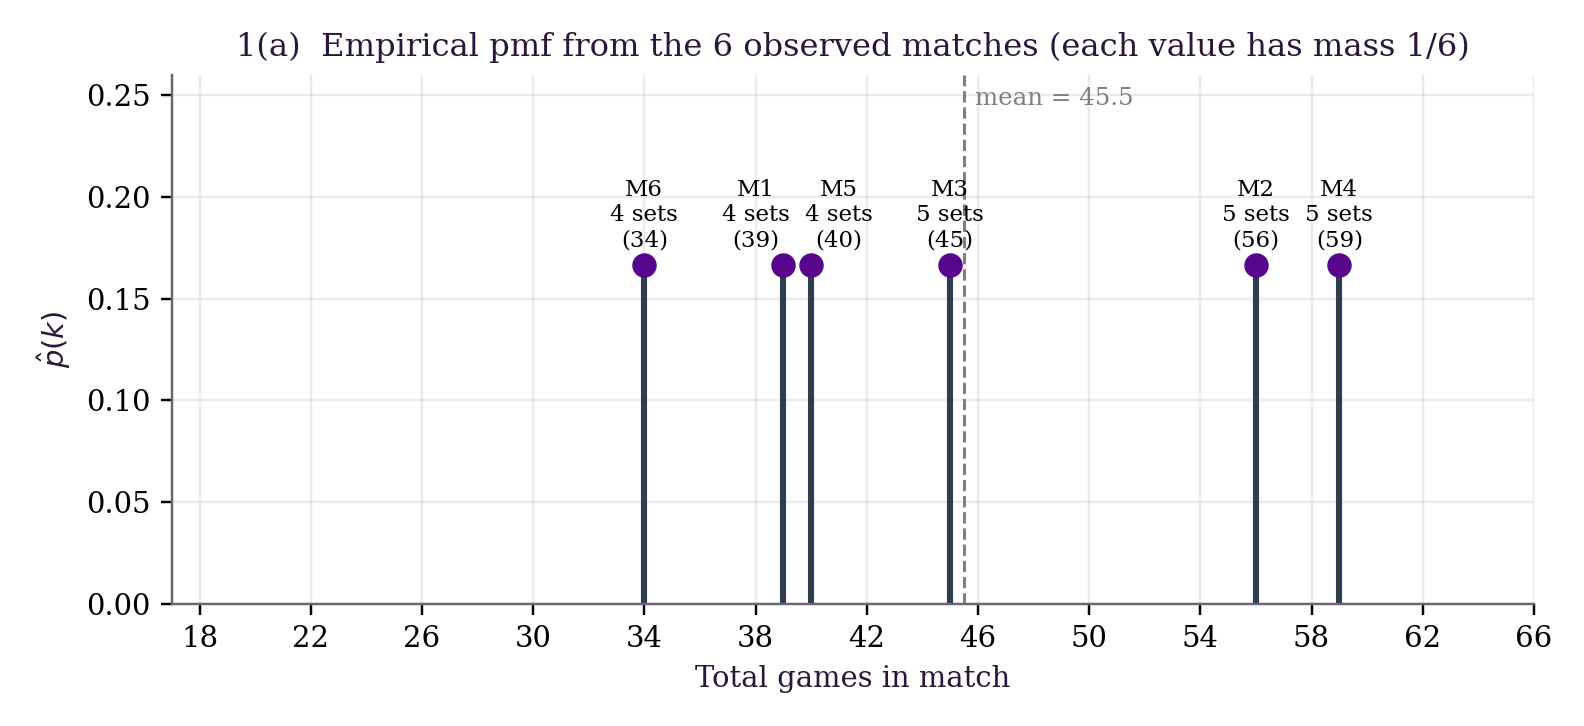
\includegraphics[width=0.92\linewidth]{fig1a.png}
  \caption{Empirical pmf. Labels give the match, number of sets, and total games.}
  \label{fig:empirical-pmf}
\end{figure}

\begin{resultbox}
\textbf{Is it reasonable?} No. The estimate is far too coarse to be credible: it says that a 40-game match has probability $1/6$ while a 41- or 42-game match is impossible, and it assigns zero probability to every value below 34 or above 59, including all straight-set, three-set results, which certainly can occur. With $n=6$, the estimated probabilities can only be multiples of $1/6$, so the estimate is dominated by sampling noise. The data give a rough indication of location (mean $45.5$, standard deviation $9.1$), but not of the distribution's shape.
\end{resultbox}

\problemPart{1(b)}{Monte Carlo estimate from the service-point data}

\textbf{Model.} Each point is an independent Bernoulli trial. Alcaraz wins a point on his serve with probability
\[
  p_A=\frac{532}{851}=0.6251,
  \qquad
  p_S=\frac{564}{911}=0.6191
\]
for Sinner, pooled over the six matches. Games are first to four points with a two-point margin, giving hold probabilities $0.786$ and $0.774$. Sets are first to six games with a two-game margin, with a seven-point tie-break at $6$--$6$ and serve pattern A, BB, AA, $\ldots$. Serve alternates every game, the first server of the match is selected by a fair coin, and matches are best of five. The simulation records the total games in $10^5$ matches.

\begin{figure}[H]
  \centering
  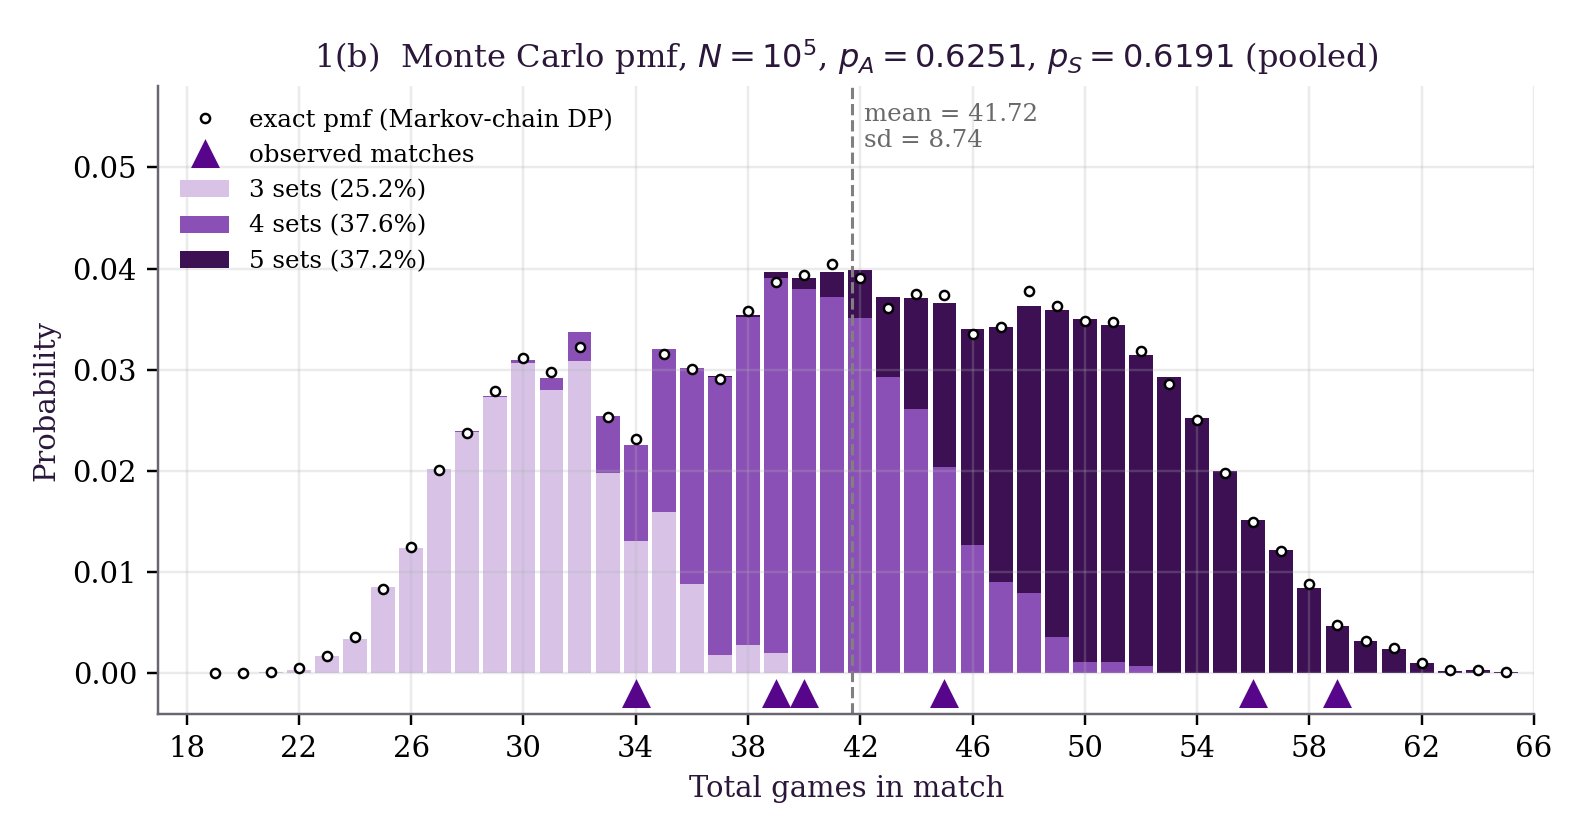
\includegraphics[width=0.94\linewidth]{fig1b.png}
  \caption{Monte Carlo pmf, colored by number of sets. Open circles show the exact pmf of the same model, computed by a Markov-chain recursion over points, games, and sets. Red triangles mark the six observed matches.}
  \label{fig:mc-pmf}
\end{figure}

\begin{resultbox}
\textbf{Is it reasonable?} Much more so than the empirical pmf in part (a). The distribution is smooth, covers the entire plausible range (simulated range $21$--$65$; theoretical range $18$--$65$), and has interpretable structure. It is a mixture of three overlapping components: three sets ($25.2\%$), four sets ($37.6\%$), and five sets ($37.2\%$). This mixture explains the bumps and dips around 30--38 games. The mean is $41.72$ games and the standard deviation is $8.74$. All six observed matches lie within the bulk of the distribution; their mid-percentiles range from $23\%$ for 34 games to $99\%$ for 59 games.
\end{resultbox}

\textbf{Caveats.} The model assumes that points are independent and identically distributed and that the serve probabilities remain the same in every match. It therefore ignores surface, form, fatigue, pressure, and momentum effects. The observed matches were somewhat longer than predicted (mean $45.5$ versus $41.7$). However, the standard error of a mean of six draws from this pmf is about $3.6$ games, so the gap is only about one standard error. Two matches, with 56 and 59 games, fall in the model's upper $5\%$ tail. Under the model, the probability of observing at least two such matches among six is approximately $0.03$, while the probability of observing no straight-set match is
\[
  0.75^6\approx0.18.
\]
Thus, the model may slightly understate how close these matches tend to be, but six observations are insufficient to reject it.

\subsection*{Validation and sensitivity}

\textbf{Validation.} The exact pmf in Figure~\ref{fig:mc-pmf} has mean $41.735$. The total-variation distance between the Monte Carlo and exact pmfs is $0.0080$, which is consistent with sampling noise at $N=10^5$. The same recursion gives
\[
  \Prob(3,4,5\text{ sets})=(0.251,0.375,0.374).
\]
This confirms that the simulation, including tie-break serve order and the change of server between sets, is implemented correctly.

\begin{figure}[H]
  \centering
  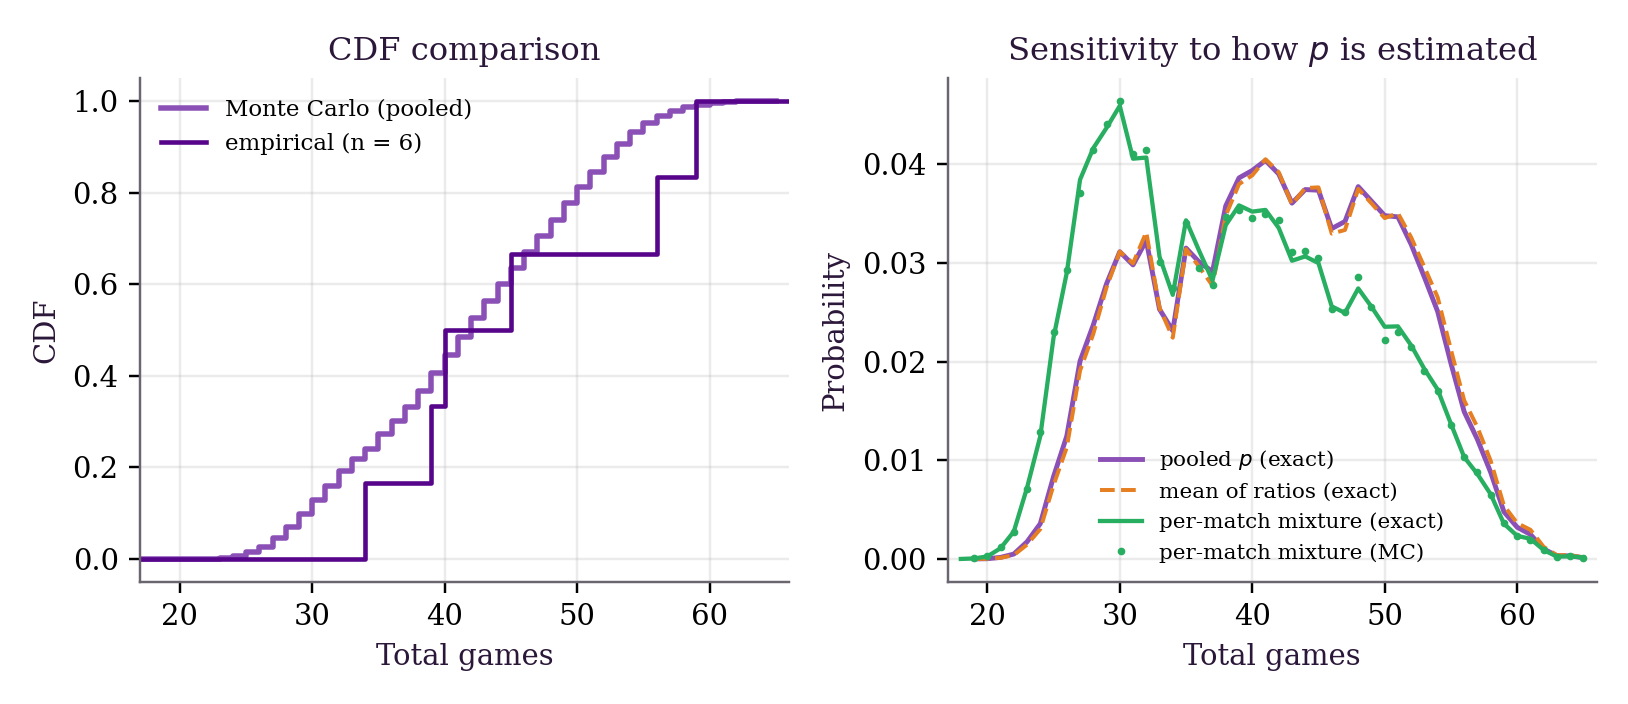
\includegraphics[width=\linewidth]{fig1c.png}
  \caption{Left: Monte Carlo CDF versus the empirical CDF of the six matches. Right: the pmf under different methods of estimating the serve probabilities.}
  \label{fig:sensitivity}
\end{figure}

Using the mean of the per-match ratios, $p_A=0.6343$ and $p_S=0.6258$, barely changes the result (mean $41.96$). A per-match mixture, in which each simulated match uses the serve rates of one randomly selected real match, shifts probability mass toward shorter matches (mean $38.7$, mode $30$). The reason is that lopsided matches such as M6, with serve probabilities $0.730$ versus $0.580$, produce quick, one-sided results. Per-match rates are partly a consequence of how each match unfolded, so pooling is the more sensible default.

\FloatBarrier
\problem{2}{Pareto distribution}

\problemPart{2(a)}{Exponential-tail comparison}

For an exponential random variable $\widetilde A$ with rate $\lambda>0$ and for $a>0$,
\[
  \Prob(\widetilde A>a)
  =\int_a^\infty \lambda e^{-\lambda t}\,dt
  =e^{-\lambda a}.
\]
Thus the tail decays exponentially in $a$. This is faster than any power law, since
\[
  a^k e^{-\lambda a}\longrightarrow 0
  \qquad\text{for every fixed }k>0.
\]

\problemPart{2(b)}{Derivation of the Pareto distribution}

We require $\widetilde A\ge m$ and
\[
  \Prob(\widetilde A>a)=Ca^{-\alpha},
  \qquad a\ge m,
\]
where $m>0$ and $\alpha>0$. The condition $\Prob(\widetilde A>m)=1$ forces $C=m^\alpha$, so
\[
F_{\widetilde A}(a)=
\begin{cases}
0, & a<m,\\[2pt]
1-\left(\dfrac{m}{a}\right)^\alpha, & a\ge m.
\end{cases}
\]
Differentiating gives the Pareto density
\[
f_{\widetilde A}(a)=
\begin{cases}
\dfrac{\alpha m^\alpha}{a^{\alpha+1}}, & a\ge m,\\[6pt]
0, & a<m.
\end{cases}
\]
It integrates to one:
\[
  \int_m^\infty \alpha m^\alpha a^{-\alpha-1}\,da
  =m^\alpha m^{-\alpha}=1.
\]
For $m=1$, the density reduces to $f(a)=\alpha/a^{\alpha+1}$.

\begin{figure}[H]
  \centering
  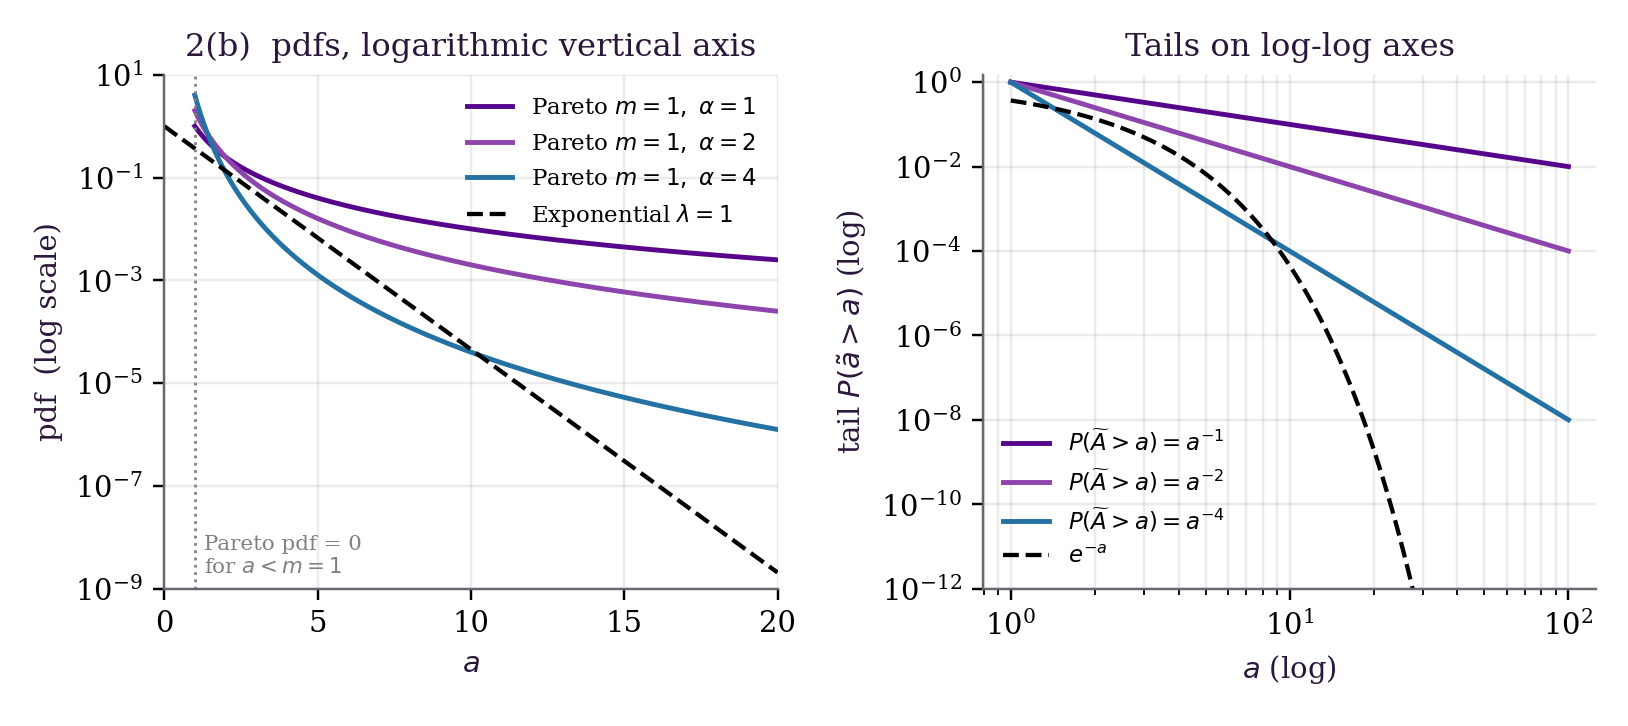
\includegraphics[width=\linewidth]{fig2.png}
  \caption{Left: Pareto densities with $m=1$ and $\alpha\in\{1,2,4\}$, together with the exponential density of rate $\lambda=1$, on a logarithmic vertical axis. Right: the corresponding tails on log--log axes, where power laws appear as straight lines of slope $-\alpha$.}
  \label{fig:pareto-comparison}
\end{figure}

\textbf{Comparison.} On a logarithmic vertical axis, the exponential density is a straight line of slope $-1$. Each Pareto density bends and flattens because
\[
  \log f(a)=\log\alpha-(\alpha+1)\log a
\]
decreases only logarithmically. Near $a=m$, the Pareto densities start high: $f(1)=\alpha$, compared with $e^{-1}\approx0.37$. For $\alpha=1$ and $\alpha=2$, the Pareto density exceeds the exponential density for every $a\ge1$. For $\alpha=4$, it falls below the exponential density between approximately $a=1.95$ and $a=10.25$, then exceeds it permanently. At $a=20$, the exponential density is about $2\times10^{-9}$, whereas the Pareto densities are $2.5\times10^{-3}$, $2.5\times10^{-4}$, and $1.2\times10^{-6}$. Every Pareto tail eventually dominates an exponential tail.

Smaller $\alpha$ produces a heavier tail. The mean $\alpha m/(\alpha-1)$ exists only for $\alpha>1$, and the variance exists only for $\alpha>2$. Thus, $\alpha=1$ has infinite mean, $\alpha=2$ has finite mean $2m$ but infinite variance, and $\alpha=4$ has both finite mean and variance.

\problemPart{2(c)}{Scale invariance of the Pareto tail}

For a Pareto variable with parameters $m>0$ and $\alpha>0$, the tail at any threshold $x\ge m$ is
\[
  \Prob(\widetilde A>x)=\left(\frac{m}{x}\right)^\alpha.
\]
Fix $s>1$ and $a\ge m$. Then both $a$ and $sa$ exceed $m$, so
\[
  \Prob(\widetilde A>a)=\left(\frac{m}{a}\right)^\alpha,
  \qquad
  \Prob(\widetilde A>sa)
  =\left(\frac{m}{sa}\right)^\alpha
  =s^{-\alpha}\left(\frac{m}{a}\right)^\alpha.
\]
Taking the ratio cancels the factor $(m/a)^\alpha$:
\[
  \boxed{
  \frac{\Prob(\widetilde A>a)}{\Prob(\widetilde A>sa)}=s^\alpha.}
\]

\begin{resultbox}
\textbf{Conclusion.} The ratio depends only on $\alpha$ and $s$, not on the threshold $a$. Multiplying the threshold by $s$ always divides the tail probability by the same factor $s^\alpha$, regardless of how far into the tail one moves. This is the defining scale-invariance, or self-similarity, of a power law. An exponential tail lacks this property because
\[
  \frac{e^{-\lambda a}}{e^{-\lambda sa}}
  =e^{\lambda(s-1)a},
\]
which grows without bound as $a$ grows. This ratio therefore provides the diagnostic used in Problem 3(c).
\end{resultbox}

\problemPart{2(d)}{Maximum-likelihood estimation of $(m,\alpha)$}

Given independent and identically distributed observations $x_1,\ldots,x_n$ with density
\[
  f(x)=\alpha m^\alpha x^{-\alpha-1}\bm{1}_{\{x\ge m\}},
\]
the likelihood is
\[
  L(m,\alpha)
  =\alpha^n m^{n\alpha}\prod_{i=1}^n x_i^{-\alpha-1}
   \bm{1}_{\{m\le x_{(1)}\}},
  \qquad x_{(1)}=\min_i x_i.
\]

\begin{enumerate}[label=\textbf{\arabic*.},leftmargin=2.1em,itemsep=7pt]
\item \textbf{Estimator of $m$.} For any fixed $\alpha>0$, the likelihood is proportional to $m^{n\alpha}$, which is strictly increasing in $m$. The indicator requires $m\le x_i$ for every $i$, equivalently $m\le x_{(1)}$. The likelihood is therefore maximized at the largest feasible value:
\[
  \boxed{\mhat=x_{(1)}=\min_i x_i.}
\]
This is a boundary maximum rather than a stationary point, so no derivative with respect to $m$ is taken. The estimator is biased upward,
\[
  \E[\mhat]=\frac{n\alpha m}{n\alpha-1}>m,
\]
although it is consistent.

\item \textbf{Estimator of $\alpha$.} Substitute $\mhat$ and write the log-likelihood as
\[
  \ell(\alpha)
  =\log L(\mhat,\alpha)
  =n\log\alpha+n\alpha\log\mhat-(\alpha+1)\sum_{i=1}^n\log x_i.
\]
Then
\[
  \ell'(\alpha)
  =\frac{n}{\alpha}-\sum_{i=1}^n\log\left(\frac{x_i}{\mhat}\right)=0,
\]
which yields
\[
  \boxed{
  \alphahat=\frac{n}{\displaystyle\sum_{i=1}^n
  \log\left(x_i/\mhat\right)}.}
\]
Since $\ell''(\alpha)=-n/\alpha^2<0$ for every $\alpha>0$, the log-likelihood is strictly concave and the stationary point is the unique global maximum. Equivalently, $\log(X_i/m)$ is exponentially distributed with rate $\alpha$, so $\alphahat$ is the reciprocal of the sample mean of the log-excesses.
\end{enumerate}

\FloatBarrier
\problem{3}{Fires}

A ``catastrophic'' fire is one that burns more than $100{,}000$ acres. Over the next 23 years at $70{,}000$ fires per year, the total number of fires is
\[
  N_{\mathrm{total}}=23\times70{,}000=1{,}610{,}000.
\]
Thus, under any fitted model, the predicted number of catastrophic fires is
\[
  1{,}610{,}000\times\widehat{\Prob}(\widetilde A>100{,}000).
\]

\problemPart{3(a)}{Nonparametric empirical model}

The empirical tail estimate is
\[
  \widehat{\Prob}(\widetilde A>100{,}000)
  =\frac{N_{\mathrm{cat},1995}}{N_{1995}},
\]
where $N_{\mathrm{cat},1995}$ is the number of 1995 fires exceeding $100{,}000$ acres. The corresponding prediction is
\[
  1{,}610{,}000\frac{N_{\mathrm{cat},1995}}{N_{1995}}.
\]

\textbf{Why it fails.}
\begin{enumerate}[label=(\roman*),leftmargin=2em,itemsep=3pt,topsep=2pt]
\item \textbf{Rare-event sampling noise.} Catastrophic fires are a tail event, so $N_{\mathrm{cat},1995}$ is very small. If no 1995 fire exceeded $100{,}000$ acres, the model assigns exactly zero probability and predicts zero catastrophic fires in 23 years. If one fire did, the estimate rests on a single observation and has relative standard error of approximately $100\%$.
\item \textbf{No extrapolation.} An empirical distribution assigns zero probability to every magnitude exceeding the largest observation, so it cannot predict an unprecedented fire.
\item \textbf{Nonstationarity.} Year-to-year weather variability and climate trends mean that one year is not representative of multi-decade tail behavior.
\end{enumerate}

\problemPart{3(b)}{Exponential model}

The exponential maximum-likelihood estimator is
\[
  \lambdahat=\frac{1}{\overline x_{1995}},
  \qquad
  \widehat{\Prob}(\widetilde A>100{,}000)
  =e^{-100{,}000/\overline x_{1995}}.
\]
Typical average fire sizes are on the order of tens or hundreds of acres, so $100{,}000/\overline x$ is in the hundreds or thousands and the estimate underflows numerically to zero. The exponential model is even less useful than the empirical estimate here: it does not merely lack information about the tail; it structurally asserts that catastrophic fires are effectively impossible. A light, exponentially decaying tail is fitted by matching the mean, while the mean of a heavy-tailed sample is driven by the many small fires. The scale-invariance property derived in Problem 2(c) is precisely what the exponential model lacks.

\problemPart{3(c)}{Tail-ratio diagnostic and model choice}

For thresholds $a_j=1,10,100,\ldots$, compute the empirical ratios
\[
  R_j=\frac{\Prob(\widetilde A>a_j)}{\Prob(\widetilde A>10a_j)}.
\]
Under the two candidate models,
\begin{align*}
\text{Exponential:}\quad
R(a)&=\frac{e^{-\lambda a}}{e^{-10\lambda a}}
     =e^{9\lambda a},
     &&\text{which grows without bound in }a,\\
\text{Pareto:}\quad
R(a)&=10^\alpha,
     &&\text{which is constant in }a.
\end{align*}
If the observed ratios satisfy $R_1\approx R_2\approx R_3$, the upper-tail data are scale invariant: increasing the threshold tenfold incurs approximately the same probability factor at every scale. This is the signature of a power law. The Pareto model is therefore the appropriate parametric choice, with
\[
  \alpha\approx\log_{10}R.
\]

\problemPart{3(d)}{Pareto fit and prediction}

Set
\[
  \mhat=\min_i x_i
  \quad\text{(or a selected tail cutoff)},
  \qquad
  \alphahat=\frac{N}{\displaystyle\sum_{i=1}^N\log(x_i/\mhat)}.
\]
Then predict
\[
  \widehat{\Prob}(\widetilde A>100{,}000)
  =\left(\frac{\mhat}{100{,}000}\right)^{\alphahat},
\]
and hence
\[
  \boxed{
  \E[\text{catastrophic fires}]
  =1{,}610{,}000
  \left(\frac{\mhat}{100{,}000}\right)^{\alphahat}.}
\]
Because a power law decays polynomially rather than exponentially, it gives a small but non-negligible probability and a realistic nonzero, finite prediction. The empirical model cannot see beyond its largest observation, while the exponential model suppresses the upper tail. The Pareto model extrapolates the tail behavior identified by the diagnostic in part (c).

\subsection*{Numerical demonstration on synthetic data}

The supplied script draws $n=5000$ acreages by inverse transform from a Pareto distribution with true parameters $\alpha=1.5$ and $m=10$, then fits both models. Its output is

\begin{lstlisting}[style=output]
m_hat      = 10.000078      (true m = 10)
alpha_hat  = 1.515540       (true alpha = 1.5)
lambda_hat = 0.035874       (= 1 / sample mean 27.876)
sample median = 15.874      sample max = 2323.6
\end{lstlisting}

\begin{figure}[H]
  \centering
  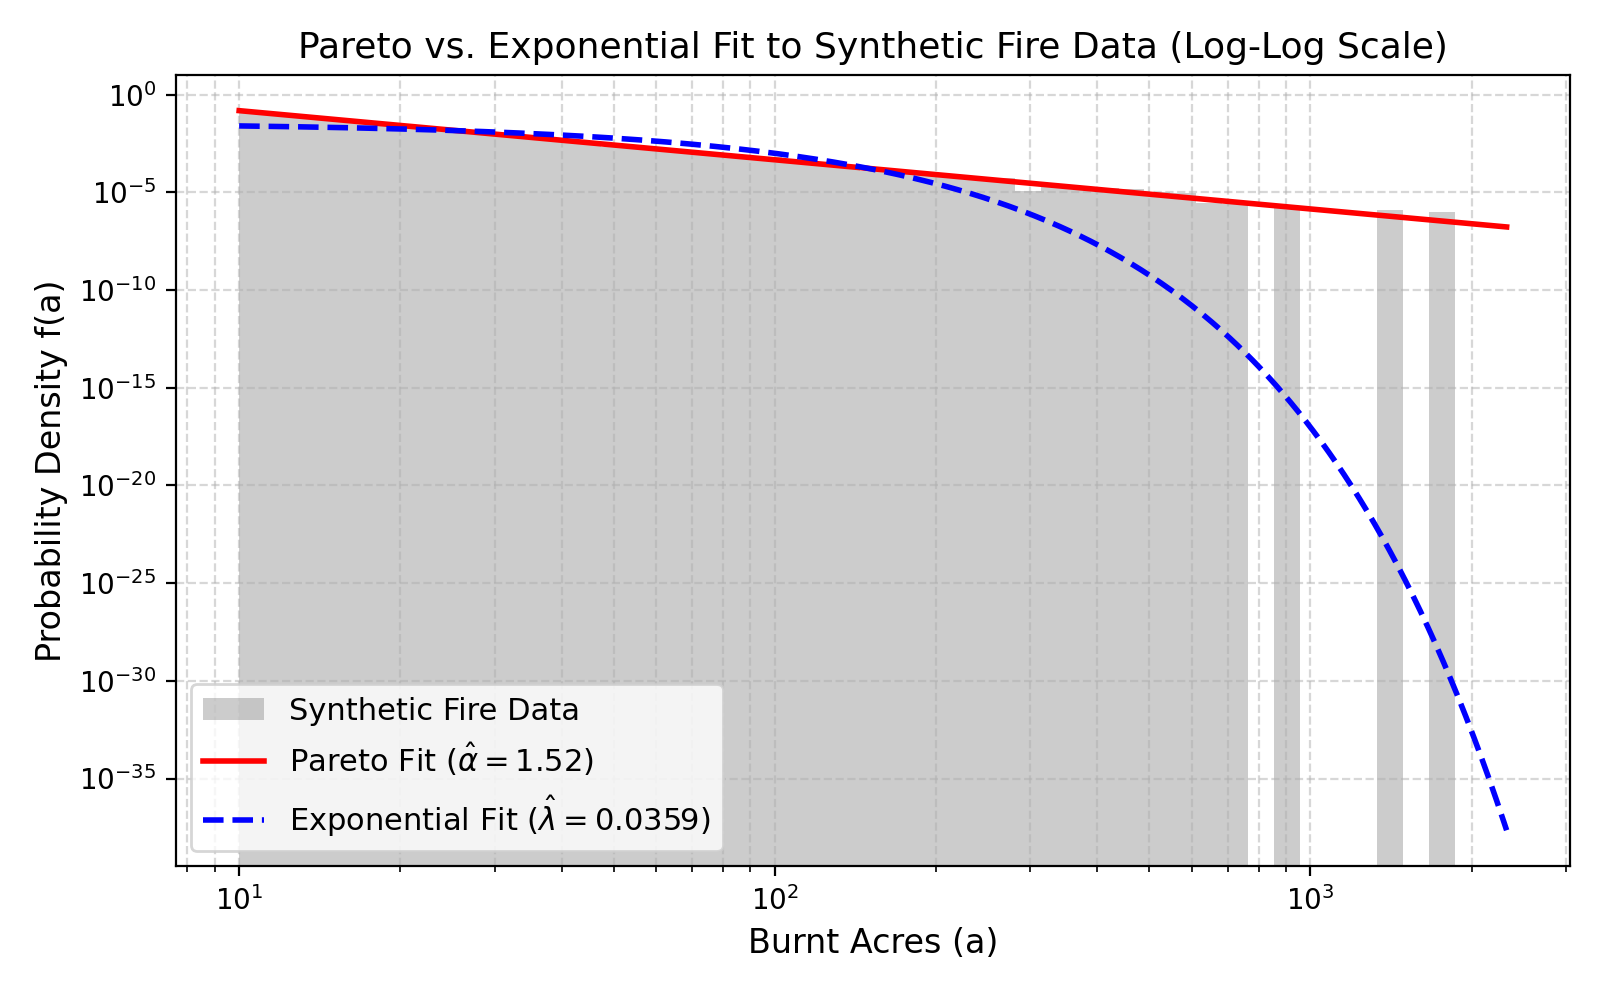
\includegraphics[width=0.86\linewidth]{fig_fire_orig.png}
  \caption{Direct log--log comparison of the fitted Pareto and unshifted exponential densities. The exponential curve forces a very low automatic vertical limit, visually flattening the histogram.}
  \label{fig:fire-original}
\end{figure}

\begin{figure}[H]
  \centering
  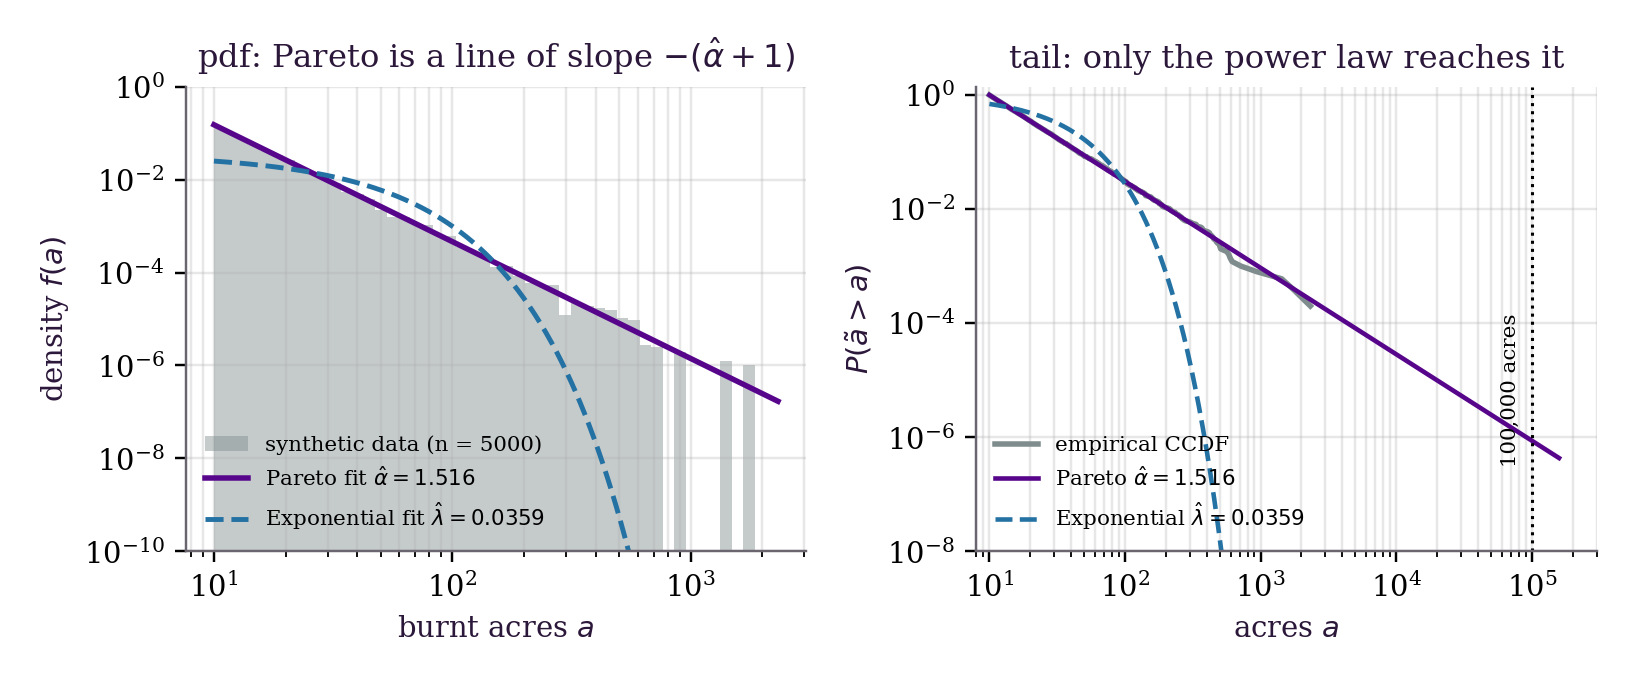
\includegraphics[width=\linewidth]{fig3.png}
  \caption{Left: the same fit with the vertical axis clipped at $10^{-10}$. On log--log axes, the Pareto density is a straight line with slope $-(\alphahat+1)=-2.52$, matching the data across three decades, while the exponential fit collapses beyond a few hundred acres. Right: complementary cumulative distribution functions extrapolated to the $100{,}000$-acre threshold.}
  \label{fig:fire-refit}
\end{figure}

\begin{figure}[H]
  \centering
  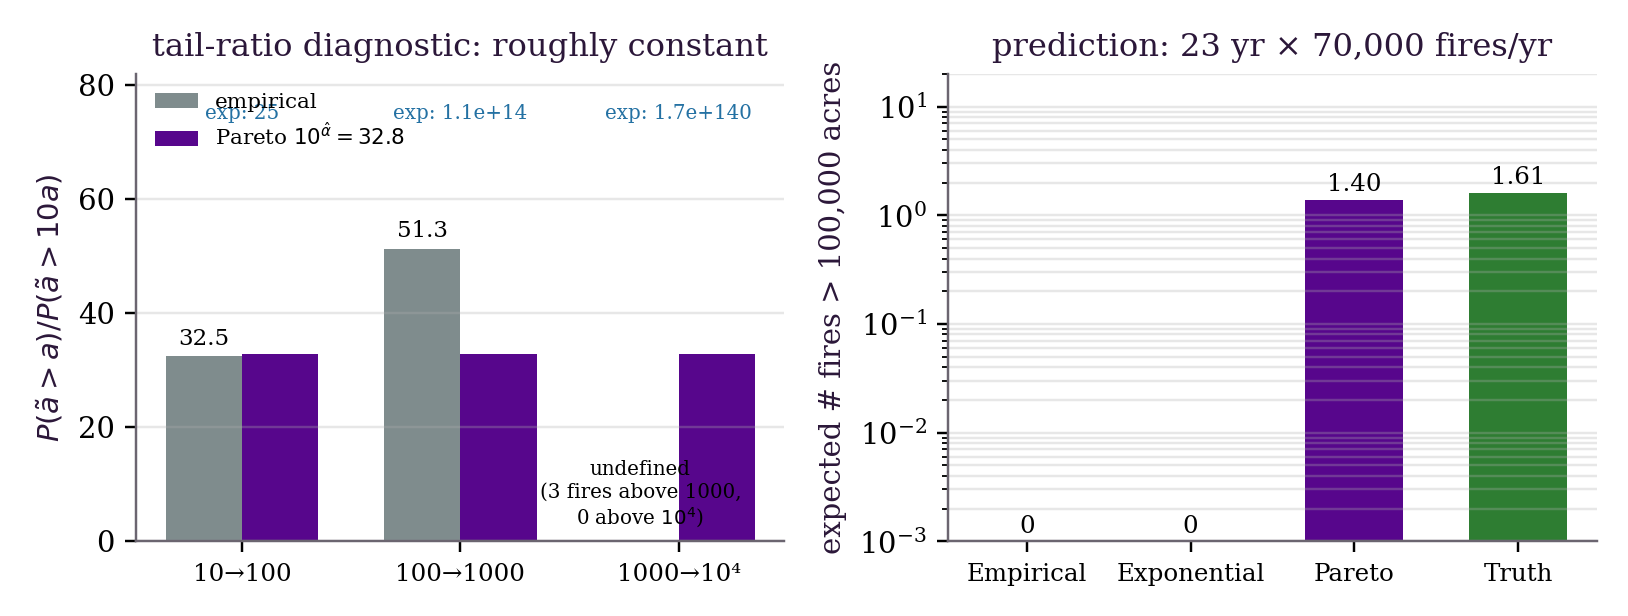
\includegraphics[width=\linewidth]{fig4.png}
  \caption{Left: the tail-ratio diagnostic from part (c). Right: the predicted number of catastrophic fires under each model.}
  \label{fig:fire-diagnostic}
\end{figure}

\begin{resultbox}
\textbf{Results.} The empirical tail ratios are $32.5$ for $10\to100$ and $51.3$ for $100\to1000$, compared with the Pareto prediction $10^{\alphahat}=32.8$; they are approximately constant, as part (c) predicts. The exponential model would require ratios of $25$, $1.1\times10^{14}$, and $1.7\times10^{140}$, missing the largest-scale behavior by more than one hundred orders of magnitude.

At the $100{,}000$-acre threshold, the Pareto fit gives $\widehat{\Prob}=8.67\times10^{-7}$ and predicts $1.40$ catastrophic fires over 23 years, compared with the truth of $1.61$ implied by the generating distribution. The exponential model gives $e^{-3587}\approx0$, and the empirical model gives zero because the largest of the 5000 samples is only about $2300$ acres. This is the central numerical conclusion of the problem.
\end{resultbox}

\begin{minipage}{\linewidth}
\textbf{Model consistency and a statistical caveat.} The code uses the same unshifted exponential model throughout:
\[
  f(a)=\lambdahat e^{-\lambdahat a},
  \qquad
  \widehat{\Prob}(\widetilde A>a)=e^{-\lambdahat a},
  \qquad
  \lambdahat=\frac{1}{\overline x}.
\]
Thus the fitted density, estimator, and catastrophic-tail calculation refer to one model. At $\alpha=1.5$ the Pareto population variance is infinite, and for $\alpha\le1$ the mean is also infinite. The sample mean of $27.9$, compared with the true mean $30$, is therefore unstable, providing an additional reason not to fit heavy tails by moment matching.
\end{minipage}

\FloatBarrier
\problem{4}{Kullback--Leibler divergence}

\subsection*{Nonnegativity via Jensen's inequality}

For probability mass functions $p$ and $q$ on a support $\mathcal A$, define
\[
  D(p\Vert q)
  =\sum_{a\in\mathcal A}p(a)
  \log\frac{p(a)}{q(a)}.
\]
Apply Jensen's inequality to the strictly concave function $g(x)=\log x$, using the weights $p(a)$, which sum to one:
\begin{align*}
  -D(p\Vert q)
  &=\sum_{a\in\mathcal A}p(a)
    \log\frac{q(a)}{p(a)}\\
  &\le
    \log\left(
      \sum_{a\in\mathcal A}p(a)\frac{q(a)}{p(a)}
    \right)\\
  &=\log\left(\sum_{a\in\mathcal A}q(a)\right)
  \le\log1=0.
\end{align*}
Therefore,
\[
  \boxed{D(p\Vert q)\ge0.}
\]
Because $\log$ is strictly concave, equality in Jensen's inequality holds only when $q(A)/p(A)$ is constant $p$-almost surely. Together with $\sum_a q(a)=1$, this constant must equal one. Hence
\[
  D(p\Vert q)=0
  \quad\Longleftrightarrow\quad
  p(a)=q(a)\quad\text{for all }a.
\]
If $q(a)=0$ while $p(a)>0$ for some $a$, the divergence is $+\infty$ by convention, consistent with the inequality.

\subsection*{KL divergence between two multivariate Gaussians}

Let
\[
  p=\mathcal N(\mu_0,\Sigma_0),
  \qquad
  q=\mathcal N(\mu_1,\Sigma_1)
\]
on $\mathbb R^d$, with positive-definite covariance matrices. Then
\[
  D(p\Vert q)=\E_p[\log p(X)]-\E_p[\log q(X)],
\]
where
\[
  \log p(x)
  =-\frac12\left[
    d\log(2\pi)+\log|\Sigma_0|
    +(x-\mu_0)^\mathsf T\Sigma_0^{-1}(x-\mu_0)
  \right],
\]
and analogously for $q$.

\textbf{Step 1.} Use $\E[Y^\mathsf TAY]=\operatorname{tr}(A\E[YY^\mathsf T])$ with $Y=X-\mu_0$, for which $\E[YY^\mathsf T]=\Sigma_0$:
\begin{align*}
\E_p\!\left[(X-\mu_0)^\mathsf T\Sigma_0^{-1}(X-\mu_0)\right]
&=\operatorname{tr}(\Sigma_0^{-1}\Sigma_0)\\
&=\operatorname{tr}(I_d)=d.
\end{align*}
Thus,
\[
  \E_p[\log p(X)]
  =-\frac12\left[d\log(2\pi)+\log|\Sigma_0|+d\right].
\]

\textbf{Step 2.} Decompose
\[
  X-\mu_1=(X-\mu_0)+(\mu_0-\mu_1)
\]
and expand the quadratic form. The cross terms vanish because $\E_p[X-\mu_0]=0$. Hence
\begin{align*}
&\E_p\!\left[(X-\mu_1)^\mathsf T\Sigma_1^{-1}(X-\mu_1)\right]\\
&\qquad=\operatorname{tr}(\Sigma_1^{-1}\Sigma_0)
 +(\mu_0-\mu_1)^\mathsf T\Sigma_1^{-1}(\mu_0-\mu_1),
\end{align*}
and therefore
\begin{align*}
\E_p[\log q(X)]
=-\frac12\bigl[&d\log(2\pi)+\log|\Sigma_1|
+\operatorname{tr}(\Sigma_1^{-1}\Sigma_0)\\
&+(\mu_1-\mu_0)^\mathsf T\Sigma_1^{-1}(\mu_1-\mu_0)
\bigr].
\end{align*}

\textbf{Step 3.} Subtract the two expectations. The $d\log(2\pi)$ terms cancel, giving
\begin{resultbox}
\[
\boxed{
D(p\Vert q)=\frac12\left[
\log\frac{|\Sigma_1|}{|\Sigma_0|}
-d
+\operatorname{tr}(\Sigma_1^{-1}\Sigma_0)
+(\mu_1-\mu_0)^\mathsf T\Sigma_1^{-1}(\mu_1-\mu_0)
\right].}
\]
\end{resultbox}

\textbf{Sanity checks.} If $\mu_0=\mu_1$ and $\Sigma_0=\Sigma_1$, then
\[
  \log1-d+\operatorname{tr}(I_d)+0=0.
\]
In one dimension, the formula reduces to
\[
  D(p\Vert q)
  =\frac12\left[
    \log\frac{\sigma_1^2}{\sigma_0^2}-1
    +\frac{\sigma_0^2}{\sigma_1^2}
    +\frac{(\mu_1-\mu_0)^2}{\sigma_1^2}
  \right].
\]
With equal means and $t=\sigma_0^2/\sigma_1^2$, this becomes
\[
  \frac12\bigl(t-1-\log t\bigr),
\]
which is nonnegative and equals zero only at $t=1$.

\textbf{Numerical check.} For a randomly generated four-dimensional pair of Gaussians, the closed form gives $D(p\Vert q)=1.7566$ nats. A Monte Carlo estimate of $\E_p[\log p-\log q]$ from $2\times10^6$ samples gives
\[
  1.7540\pm0.0058
\]
using three standard errors. The reverse divergence is $D(q\Vert p)=1.4244$, confirming that KL divergence is asymmetric and therefore is not a metric.

\begin{figure}[H]
  \centering
  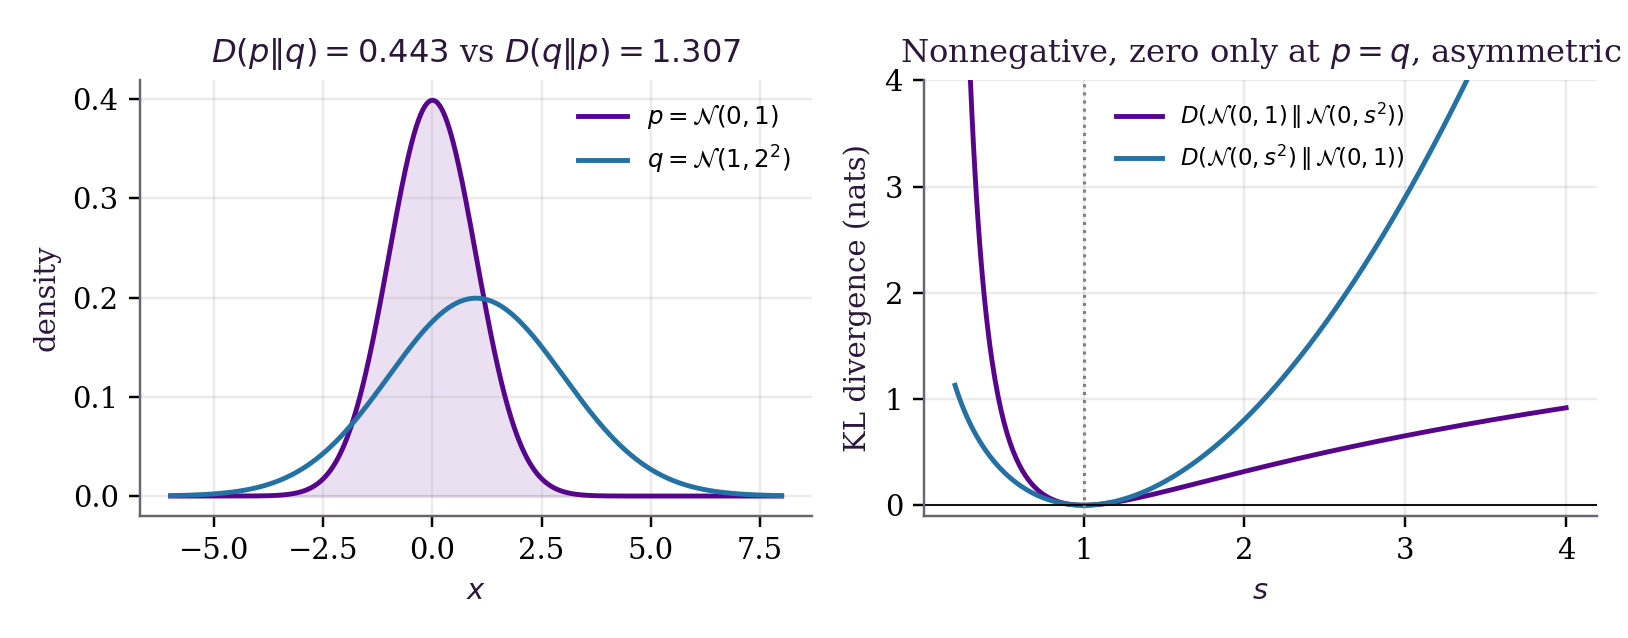
\includegraphics[width=\linewidth]{fig5.png}
  \caption{Left: two Gaussians and their two divergences, illustrating asymmetry. Right: both divergence directions between $\mathcal N(0,1)$ and $\mathcal N(0,s^2)$. Each is nonnegative and zero only at $s=1$; the forward direction grows logarithmically as $s\to\infty$, while the reverse direction grows like $s^2/2$.}
  \label{fig:gaussian-kl}
\end{figure}

\problemPart{4(a)}{Maximum likelihood is KL minimization}

Let $X=\{x_1,\ldots,x_n\}$ be independent observations taking values in a discrete support $\mathcal A$, and let
\[
  n_a=\#\{i:x_i=a\}.
\]
The empirical pmf is
\[
  p_X(a)=\frac{n_a}{n},
  \qquad
  \sum_{a\in\mathcal A}p_X(a)=1.
\]
For a parametric model $p_\theta$, the likelihood can be grouped by outcomes:
\[
  L(\theta)
  =\prod_{i=1}^n p_\theta(x_i)
  =\prod_{a\in\mathcal A}p_\theta(a)^{n_a}.
\]
Taking logarithms and dividing by $n$,
\[
  \frac1n\log L(\theta)
  =\sum_{a\in\mathcal A}\frac{n_a}{n}\log p_\theta(a)
  =\sum_{a\in\mathcal A}p_X(a)\log p_\theta(a).
\]
Now split the divergence between the empirical and model distributions:
\begin{align*}
D(p_X\Vert p_\theta)
&=\sum_a p_X(a)\log p_X(a)
  -\sum_a p_X(a)\log p_\theta(a)\\
&=-H(p_X)-\frac1n\log L(\theta),
\end{align*}
where
\[
  H(p_X)=-\sum_a p_X(a)\log p_X(a)
\]
is the empirical entropy, which depends only on the observed data and is constant in $\theta$. Rearranging gives
\[
  \frac1n\log L(\theta)
  =-H(p_X)-D(p_X\Vert p_\theta).
\]
Consequently,
\begin{resultbox}
\[
  \boxed{
  \operatorname*{arg\,max}_\theta L(\theta)
  =\operatorname*{arg\,min}_\theta D(p_X\Vert p_\theta).}
\]
The two objectives differ only by an additive constant and a sign. Maximizing likelihood is therefore exactly equivalent to minimizing KL divergence from the empirical distribution to the model.
\end{resultbox}

Two consequences follow. First, nonnegativity implies
\[
  \frac1n\log L(\theta)\le-H(p_X),
\]
with equality only if the model can reproduce the empirical pmf exactly. Thus, the empirical pmf is the maximum-likelihood fit within the unrestricted family. Second, the direction of the divergence is $D(p_X\Vert p_\theta)$, not its reverse. If $p_X(a)>0$ for an observed outcome but $p_\theta(a)=0$, the model incurs infinite divergence and has zero likelihood.

\problemPart{4(b)}{Second-order approximation: a weighted sum of squares}

The second-order Taylor expansion of $\log u$ about $u_0=1$ is
\[
  \log u=(u-1)-\frac12(u-1)^2+O\bigl((u-1)^3\bigr).
\]
Using $\log(a/b)=-\log(b/a)$, rewrite the divergence as
\[
  D(p_X\Vert p_\theta)
  =-\sum_a p_X(a)\log u_a,
  \qquad
  u_a=\frac{p_\theta(a)}{p_X(a)}.
\]
When $p_\theta$ is close to $p_X$, every $u_a$ is close to one, and
\[
  D(p_X\Vert p_\theta)
  \approx
  -\sum_a p_X(a)(u_a-1)
  +\frac12\sum_a p_X(a)(u_a-1)^2.
\]

\textbf{Linear term.} Since
\[
  p_X(a)(u_a-1)=p_\theta(a)-p_X(a),
\]
and both pmfs sum to one,
\[
  \sum_a p_X(a)(u_a-1)
  =\sum_a p_\theta(a)-\sum_a p_X(a)=0.
\]

\textbf{Quadratic term.} We have
\[
  p_X(a)(u_a-1)^2
  =\frac{\bigl(p_\theta(a)-p_X(a)\bigr)^2}{p_X(a)}.
\]
Therefore,
\begin{resultbox}
\[
  \boxed{
  D(p_X\Vert p_\theta)
  \approx\frac12\sum_{a\in\mathcal A}
  \frac{\bigl(p_\theta(a)-p_X(a)\bigr)^2}{p_X(a)}.}
\]
Near the empirical distribution, maximum likelihood is locally a weighted least-squares fit with weights $w(a)=1/p_X(a)$.
\end{resultbox}

Rare outcomes receive the largest weights. A discrepancy of $0.01$ on an outcome with empirical probability $0.02$ costs 25 times as much as the same discrepancy on an outcome with probability $0.5$. This explains why likelihood-based fitting is sensitive to the tail, precisely the behavior needed in Problem 3 and missed by moment matching.

In terms of observed counts $O_a=np_X(a)$ and expected counts $E_a=np_\theta(a)$, the approximation becomes
\[
  D(p_X\Vert p_\theta)
  \approx\frac{1}{2n}\sum_a\frac{(O_a-E_a)^2}{O_a}.
\]
Thus $2nD(p_X\Vert p_{\widehat\theta})$, the likelihood-ratio statistic $G^2$, and the corresponding chi-square statistic agree to leading order and share the same asymptotic chi-square distribution.

\textbf{Precision point.} The denominator in the displayed approximation is the empirical probability $p_X(a)$, giving Neyman's modified chi-square rather than Pearson's statistic, whose denominator is the expected probability $p_\theta(a)$. Expanding the reverse divergence $D(p_\theta\Vert p_X)$ gives Pearson's form. The two differ only at third order in $p_\theta-p_X$ and are asymptotically equivalent, although they are not the same statistic. The approximation also requires $p_X(a)>0$ for every outcome in the support: an outcome with zero empirical probability produces an infinite weight, mirroring the empirical model's failure on unobserved extremes in Problem 3(a).

\subsection*{Numerical verification}

Fit a $\operatorname{Binomial}(K=6,\theta)$ model to $n=800$ observations generated at $\theta=0.4$. The grid maximizer of $n^{-1}\log L$ and the grid minimizer of $D(p_X\Vert p_\theta)$ are both $0.3883$, matching the closed-form estimator
\[
  \widehat\theta=\frac{\overline x}{K}=0.3881.
\]
The identity
\[
  \frac1n\log L+D+H=0
\]
holds throughout the grid to $6.7\times10^{-16}$, at machine precision, with $H(p_X)=1.5781$ nats.

\begin{figure}[H]
  \centering
  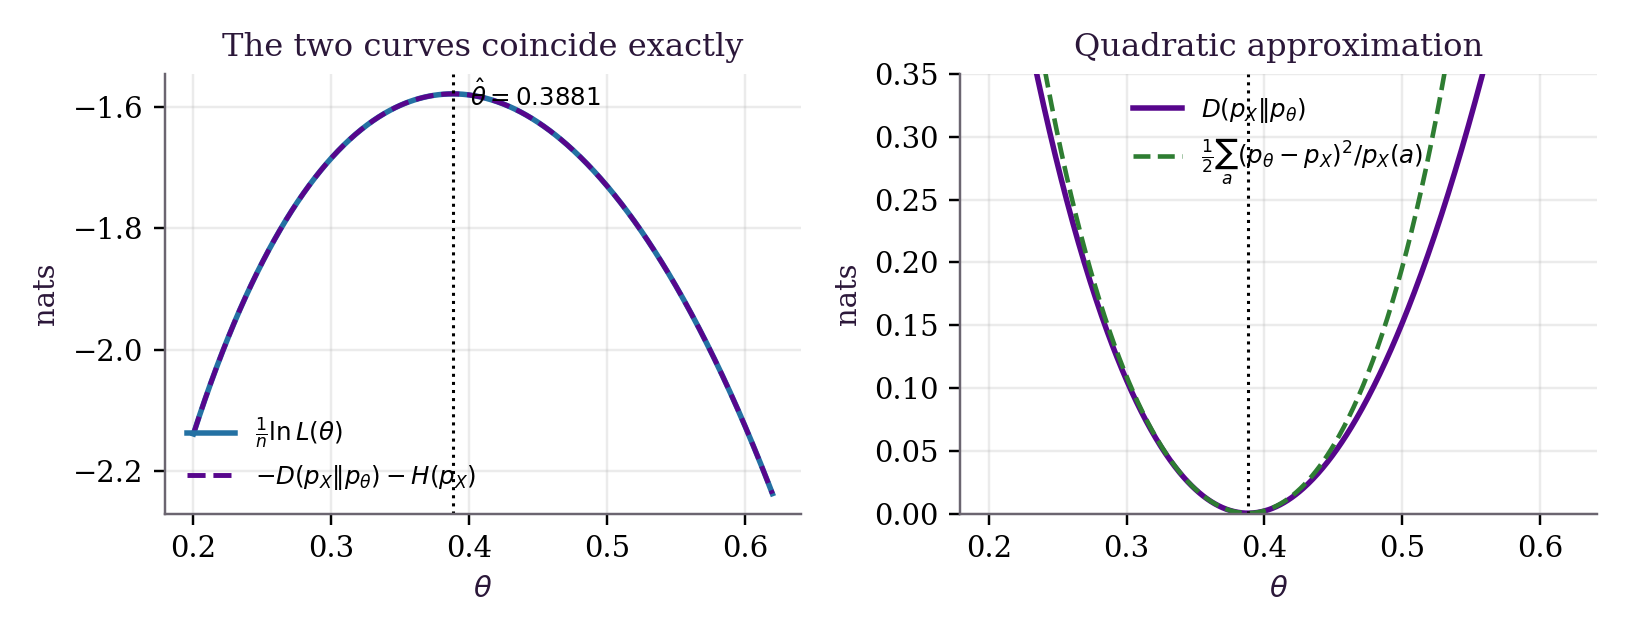
\includegraphics[width=\linewidth]{fig6.png}
  \caption{Left: average log-likelihood and $-D-H$ as functions of $\theta$ coincide, so they share a maximizer. Right: KL divergence and its weighted least-squares approximation near the optimum.}
  \label{fig:likelihood-kl}
\end{figure}

\begin{figure}[H]
  \centering
  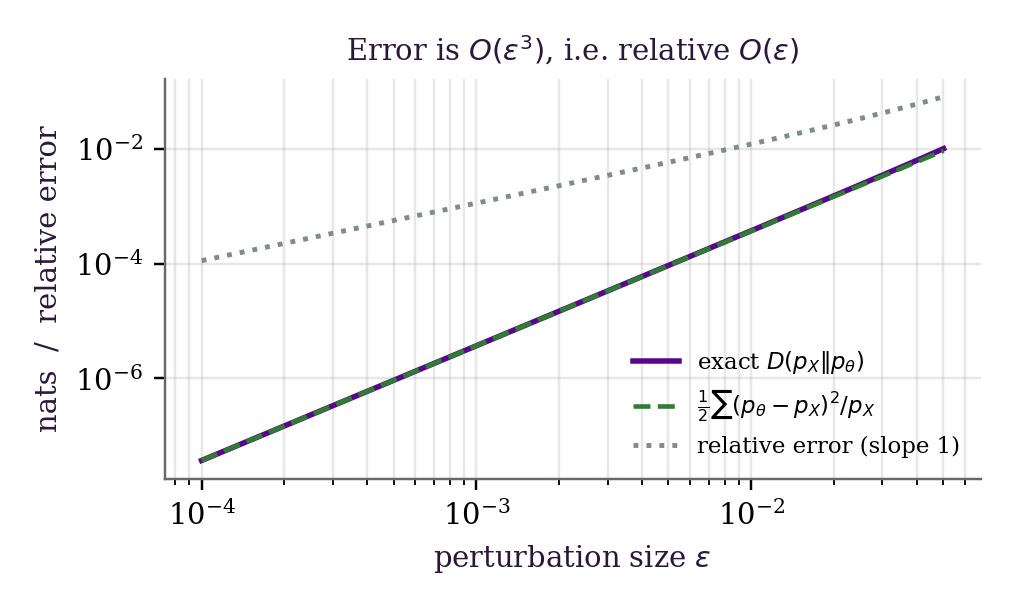
\includegraphics[width=0.72\linewidth]{fig7.png}
  \caption{A five-outcome pmf is perturbed by $\varepsilon d$. The exact divergence is compared with the quadratic approximation. The relative error decreases linearly in $\varepsilon$ with fitted slope $1.04$, confirming that the neglected term is third order.}
  \label{fig:kl-taylor-error}
\end{figure}

The approximation error behaves as predicted. At $\varepsilon=10^{-3}$, the relative error is $1.06\times10^{-3}$, and the fitted log--log slope of relative error against $\varepsilon$ is $1.04$. Hence the absolute error is $O(\varepsilon^3)$, as required by the third-order Taylor term. Away from the optimum the approximation visibly deteriorates: in the right panel of Figure~\ref{fig:likelihood-kl}, it overshoots for $\theta$ well above $\widehat\theta$, which is the expected behavior of a local expansion.

\end{document}
